\documentclass[tikz,border=3.14mm]{standalone}
\usepackage{tikz}
\usetikzlibrary{calc}
\usetikzlibrary{intersections} % name path需要使用

\begin{document}
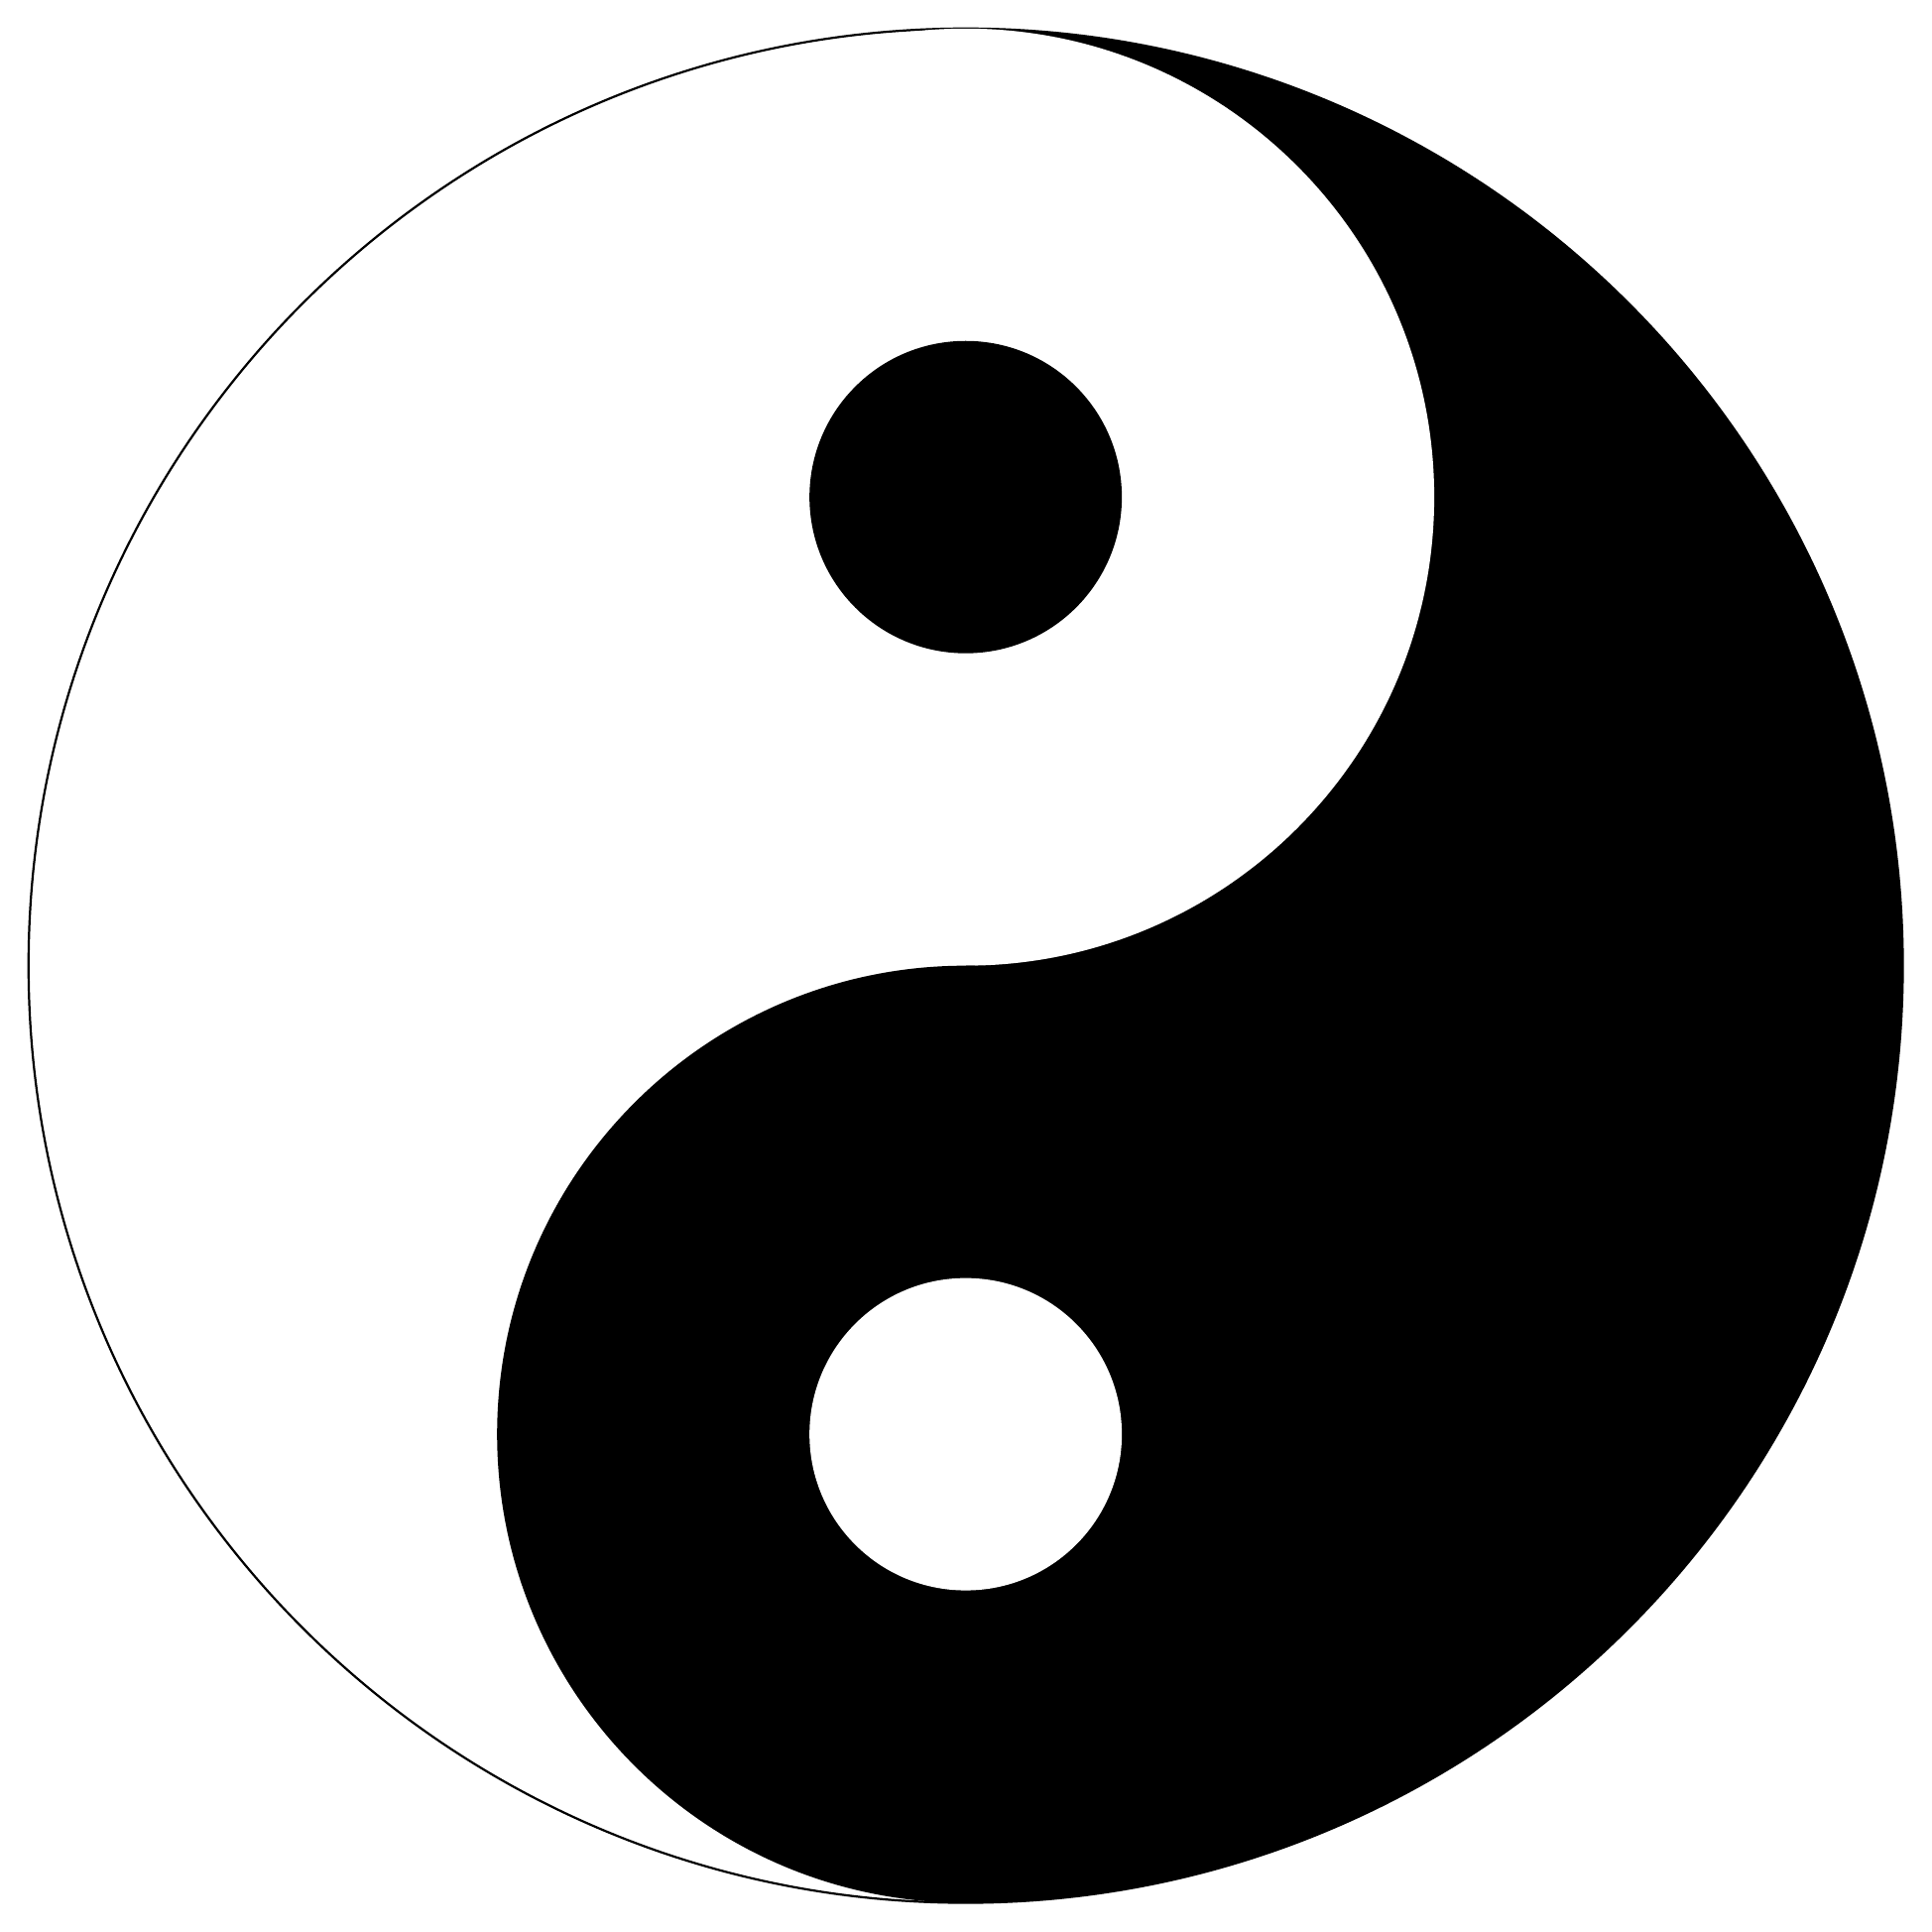
\begin{tikzpicture}
\def\r{12}

% 绘制阴阳鱼的大圆
\draw [thick](0,0) circle(\r);
\clip (0,0) circle(\r);
% 绘制黑色部分(右半圆涂黑)
\fill [black] (0, -\r) rectangle (\r, \r);
% 绘制鱼头鱼尾
% 黑色半圆中画大圆半径1/2的白色实心圆
\fill [white] (90:{1/2*\r}) circle({1/2*\r});
% 白色半圆中画大圆半径1/2的黑色实心圆
\fill [black] (-90:{1/2*\r}) circle({1/2*\r});
% 绘制鱼眼,1/6半径
\fill [black] (90:{1/2*\r}) circle({1/6*\r});
\fill [white] (-90:{1/2*\r}) circle({1/6*\r});

\end{tikzpicture}
\end{document}
